\chapter{Bagaimana LLM Bekerja?}
\label{chap:how_it_works}

Pernahkah Anda bertanya-tanya, bagaimana ChatGPT bisa menulis puisi yang masuk akal, atau kode Python yang hampir benar? Apakah ia benar-benar berpikir? Apakah ia memiliki kesadaran?

Jawabannya: **Tidak**.

Model Bahasa Besar (Large Language Models atau LLM) pada dasarnya adalah mesin prediksi kata yang sangat canggih.

\section{Analogi Burung Beo Probabilistik}

Bayangkan sebuah burung beo yang telah mendengarkan jutaan percakapan manusia. Burung beo ini sangat cerdas, tetapi ia tidak benar-benar memahami arti kata "cinta" atau "keadilan". Ia hanya tahu bahwa setelah kata "Aku", kemungkinan besar kata berikutnya adalah "cinta", "suka", atau "benci", tetapi jarang sekali "meja".

LLM seperti GPT-4 bekerja dengan prinsip yang sama, tetapi dengan skala data yang jauh lebih besar. Ia mempelajari pola statistik dari miliaran kalimat di internet.

\begin{quote}
"Kecerdasan" yang kita lihat adalah ilusi yang muncul dari statistik yang sangat kompleks.
\end{quote}

\section{Tokenisasi: Cara AI Membaca}

\begin{figure}[h]
    \centering
    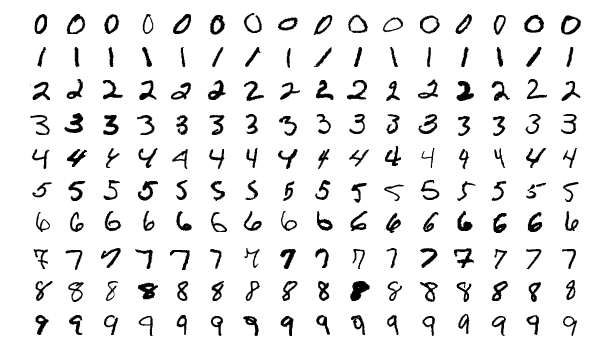
\includegraphics[width=0.8\textwidth]{ai_literacy_guide/images/computer_vision.png}
    \caption{Komputer melihat gambar sebagai matriks angka (pixel values), mirip dengan cara ia melihat teks sebagai token.}
\end{figure}

Komputer tidak memahami huruf atau kata seperti kita. Mereka hanya mengerti angka.

Ketika Anda mengetik "Saya suka AI", komputer mengubahnya menjadi serangkaian angka yang disebut **Token**.

\begin{codeblock}
Input: "Saya suka AI"

Tokenisasi: [482, 1209, 102]
(Angka ini adalah representasi matematis dari kata-kata tersebut)
\end{codeblock}

Satu token bisa berupa satu kata penuh ("suka"), sebagian kata ("ing" dalam "working"), atau bahkan satu huruf. Secara kasar, 1000 token setara dengan 750 kata bahasa Inggris.

\begin{tipbox}
\textbf{Mengapa ini penting?}
Karena LLM memiliki batas "Context Window" (jendela konteks) yang dihitung dalam token, bukan kata. Jika Anda memberikan dokumen yang terlalu panjang, AI akan "lupa" bagian awal karena tokennya melebihi kapasitas memori jangka pendeknya.
\end{tipbox}

\section{Prediksi Kata Berikutnya (Next Token Prediction)}

Inti dari cara kerja LLM adalah permainan tebak-tebakan. Ia dilatih dengan cara menyembunyikan kata terakhir dari sebuah kalimat dan diminta menebaknya.

\begin{itemize}
    \item \textbf{Input:} "Ibu pergi ke pasar membeli ..."
    \item \textbf{AI Menebak:}
    \begin{itemize}
        \item sayur (60\%)
        \item buah (20\%)
        \item baju (10\%)
        \item mobil (0.001\% - sangat tidak mungkin)
    \end{itemize}
\end{itemize}

AI memilih kata dengan probabilitas tertinggi (atau terkadang mengambil risiko kecil untuk variasi, yang disebut \textit{Temperature}).

\section{Halusinasi: Ketika AI Berbohong}

Karena LLM hanya memprediksi kata berdasarkan pola statistik, ia tidak memiliki konsep "kebenaran" atau "fakta". Ia hanya peduli pada apa yang terdengar \textit{masuk akal} secara linguistik.

Jika Anda bertanya tentang "Raja Indonesia tahun 1990", AI mungkin akan mengarang nama yang terdengar sangat Indonesia dan meyakinkan, padahal Indonesia adalah republik. Fenomena ini disebut **Halusinasi**.

\begin{exercisebox}
\textbf{Demonstrasi Halusinasi:}

Coba tanyakan pada ChatGPT pertanyaan berikut (atau yang serupa):
\textit{"Sebutkan daftar 5 buku tentang filsafat Jawa yang ditulis oleh Elon Musk."}

Elon Musk tidak pernah menulis buku filsafat Jawa. Namun, model AI yang lama mungkin akan dengan percaya diri mengarang judul-judul buku yang terdengar akademis.

\textbf{Pelajaran:} Jangan pernah percaya 100\% pada output AI tanpa verifikasi, terutama untuk fakta spesifik.
\end{exercisebox}

\section{Training Data}

Dari mana AI mendapatkan pengetahuannya?

\begin{itemize}
    \item **Common Crawl:** Arsip besar halaman web dari seluruh internet.
    \item **Wikipedia:** Ensiklopedia multibahasa.
    \item **Buku Digital:** Ribuan buku fiksi dan non-fiksi (Project Gutenberg, dll).
    \item **Kode Program:** Repository publik seperti GitHub (untuk kemampuan coding).
\end{itemize}

Data ini kemudian "dibersihkan" (cleaning) dan digunakan untuk melatih model selama berbulan-bulan menggunakan ribuan GPU. Proses ini disebut **Pre-training**. Setelah itu, model dilatih ulang dengan bantuan manusia untuk membuatnya lebih aman dan bermanfaat, proses yang disebut **Fine-tuning** (RLHF - Reinforcement Learning from Human Feedback).
